\section{Endliche Drehgruppen im dreidimensionalen Raum}
\begin{bem}
 Sei $W$ ein Untervektorraum mit $\dim W = 2$ im Vektorraum V mit $\dim V = 3$. Wenn $R$ eine Drehung in $\mathcal{O}(W)$ ist, dann kann $R$ zu einer Drehung in $\mathcal{O}(V)$ erweitert werden. Dazu wählen wir eine Basis $\{x_1,x_2,x_3\}$ von $V$ mit $x_1 \in W^{\perp}$ und $x_2,x_3 \in W$, sodass die Matrix $R$ durch \begin{center}
                                                                                                                                                                                                                                                                                                                                 $A=\begin{pmatrix}                                                                                                                                                                                                                                                                                                                                     
   1 && 0 && 0 \\
   0 && \cos(\theta) && -\sin(\theta) \\
   0 && \sin(\theta) && \cos(\theta)
   \end{pmatrix}
$                                                                                                                                                                                                                                                                                                                         \end{center}
repräsentiert wird.
\end{bem}
\begin{bem}
 Wenn wir jede Transformation $T$ aus einer Diederuntergruppe $\mathcal{H}^n_2$ zu einer Drehung in $\mathcal{O}(V)$ erweitern, dann erhalten wir eine Menge von Drehungen die eine Untergruppe von $\mathcal{O}(V)$ bildet und diese Untergruppe ist isomorph zu $\mathcal{H}^n_2$. Wir bezeichnen sie als Diedergruppe $\mathcal{H}^n_3$.
\end{bem}
\subsection{Platonische Körper}
 Da endliche Untergruppen von $\OR{2}$ Symmetriegruppen von regelmäßigen Polygonen sind, ist es naheliegend, dass wir uns nun mit regelmäßigen Polyedern beschäftigen. Es gibt genau 5 regelmäßige Polyeder, die sogenannten platonischen Körper. 
 
 Wenn wir ein regelmäßiges Polyeder am Ursprung des $\mathbb{R}^3$ ausrichten, dann sind die Drehungen die das Polyeder wieder in sich überführen eine endliche Untergruppe von $\OR{3}$. Auf diese Art entstehen drei unterschiedliche endliche Gruppen von Drehungen, denn der Würfel besitzt die gleiche Menge von Drehungen wie das Oktaeder und das Ikosaeder besitzt die gleiche Menge von Drehungen wie das Dodekaeder. Die folgende Illustration verdeutlicht warum dies der Fall ist.
 \\  \\
 \begin{center}
 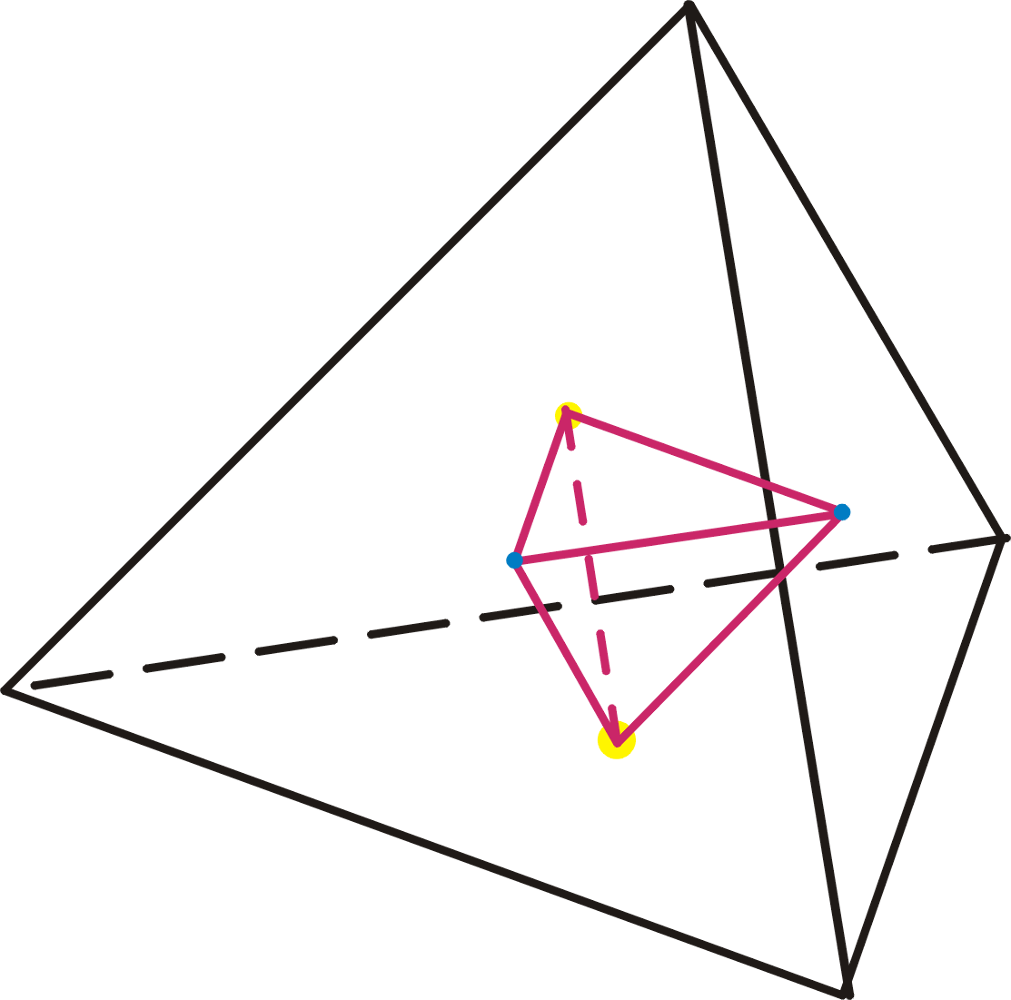
\includegraphics[height=110px]{./Grafiken/Duality_Tetra-Tetra.png} \ \
 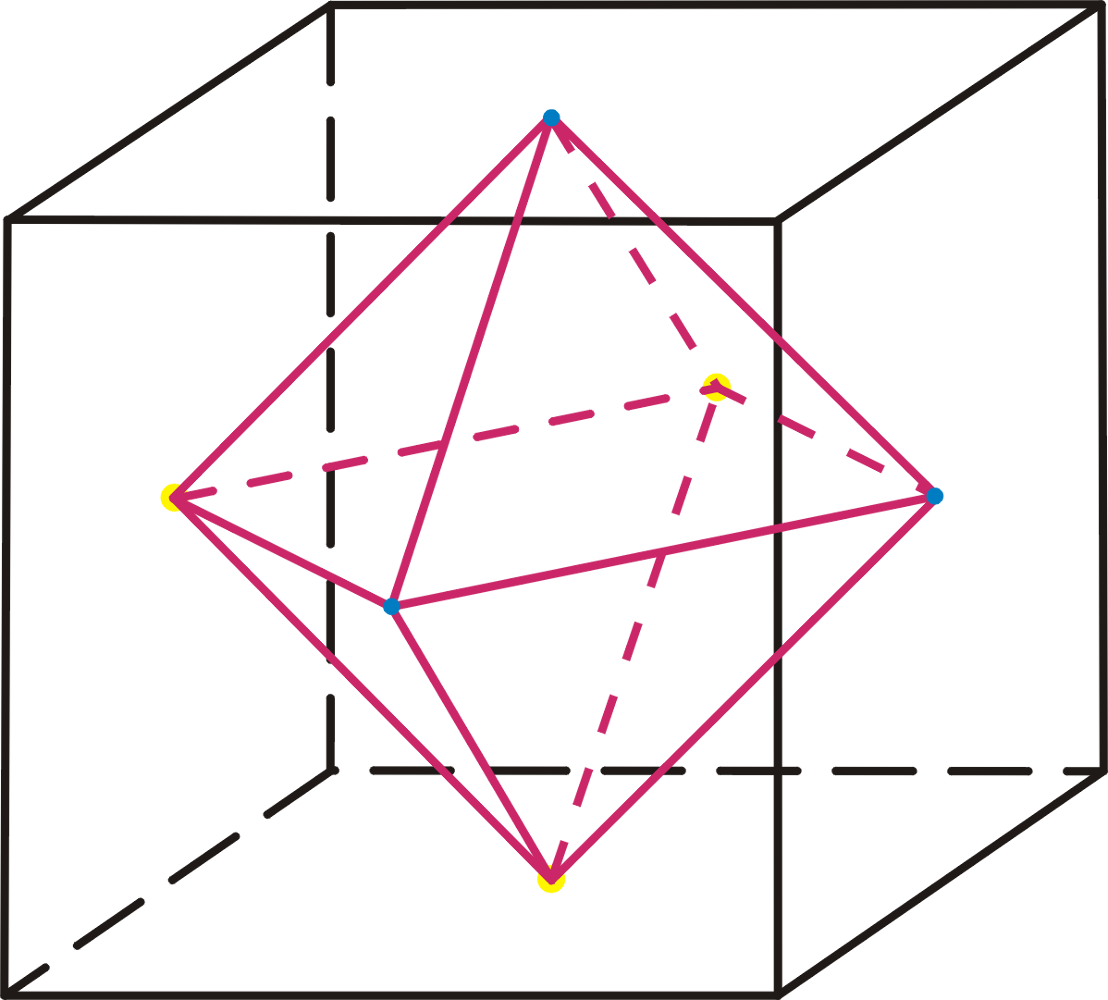
\includegraphics[height=110px]{./Grafiken/Duality_Hexa-Okta.png} \ \
 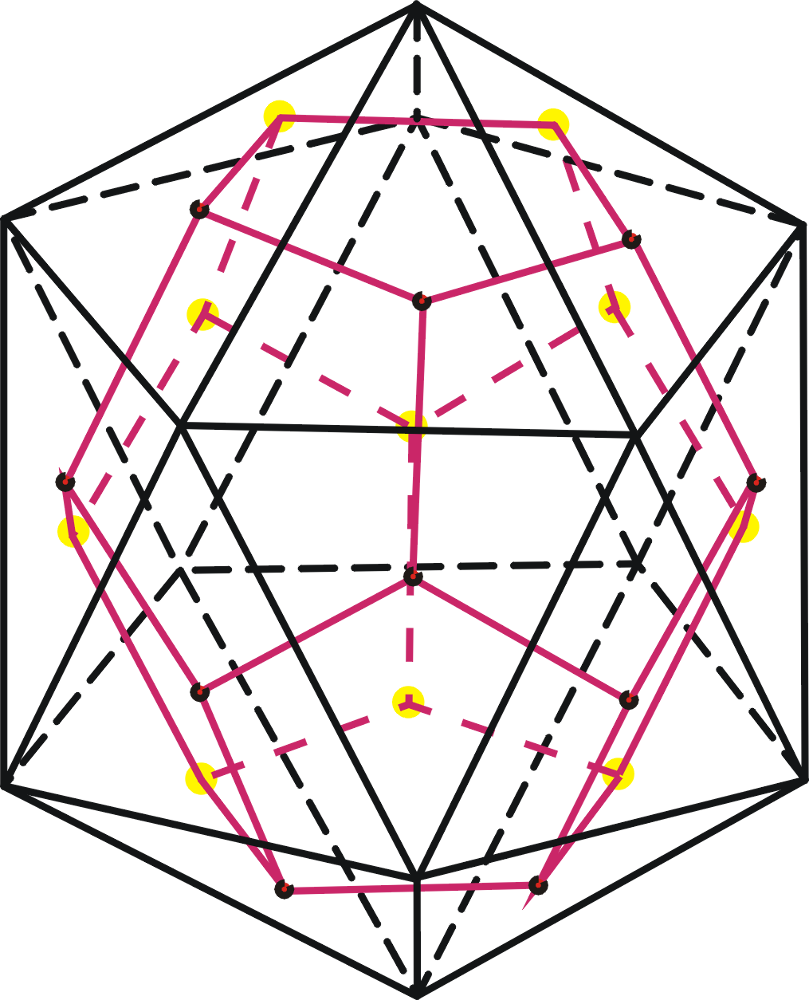
\includegraphics[height=110px]{./Grafiken/Duality_Iko-Dodek.png}
 \end{center}
 \newpage
Aus der Skizze lassen sich auch die Drehungen, die die Körper in sich überführen, leicht ablesen. Im nächsten Abschnitt nehmen wir an, dass die Schwerpunkte der Körper im Ursprung vom $\mathbb{R}^3$ liegen.

Zunächst betrachten wir die Untergruppe $\mathcal{T}$ der Drehungen von $\OR{3}$ des Tetraeders. Diese enthält
\begin{itemize}
  \item die Identität
  \item 8 Drehungen, um die Drehachsen zwischen einem Eckpunkte und dem Mittelpunkt der gegenüberliegenden Seite mit Drehwinkel $\frac{2}{3}\pi,\frac{4}{3}\pi$
  \item 3 Drehungen, um die Drehachsen zwischen den Mittelpunkten zweier gegenüberliegender Kanten mit Drehwinkel $\pi$
\end{itemize}
Es gilt somit $|\mathcal{T}|=4 \cdot 2 + 3 \cdot 1 +1 = 12$

Als nächstes betrachen wir die Untergruppe $\mathcal{W}$ der Drehungen von $\OR{3}$ des Würfels. Diese enthält
\begin{itemize} 
  \item die Identität
  \item 9 Drehungen, um die Drehachsen zwischen den Mittelpunkten zweier gegenüberliegender Seiten mit Drehwinkel $\frac{1}{2}\pi,\pi,\frac{3}{2}\pi$
  \item 8 Drehungen, um die Drehachsen zwischen zwei gegenüberliegenden Eckpunkten mit Drehwinkel $\frac{2}{3}\pi,\frac{4}{3}\pi$
  \item 6 Drehungen, um die Drehachsen zwischen den Mittelpunkten zweier gegenüberliegenden Kanten mit Drehwinkel $\pi$
\end{itemize}
Es gilt somit $|\mathcal{W}|=6 \cdot 1 + 4 \cdot 2 + 3 \cdot 3 +1 = 24$

Zuletzt betrachen wir die Untergruppe $\mathcal{I}$ der Drehungen von $\OR{3}$ des Ikosaeders. Diese enthält
\begin{itemize} 
  \item die Identität
  \item 24 Drehungen, um die Drehachsen zwischen zwei gegenüberliegendenden Eckpunkten mit Drehwinkel $\frac{2}{5}\pi,\frac{4}{5}\pi,\frac{6}{5}\pi,\frac{8}{5}\pi$
  \item 20 Drehungen, um die Drehachsen zwischen den Mittelpunkten zweier gegenüberliegender Seiten mit Drehwinkel $\frac{2}{3}\pi,\frac{4}{3}\pi$
  \item 15 Drehungen, um die Drehachsen zwischen den Mittelpunkten zweier gegenüberliegender Kanten mit Drehwinkel $\pi$
\end{itemize}
Es gilt somit $|\mathcal{I}|=15 \cdot 1 + 10 \cdot 2 + 6 \cdot 4 +1 = 60$
\begin{defi}
 Sei $E_3 \neq T \in \OR{3}$ eine Drehung, dann hat $T$ genau zwei Fixpunkte auf der Einheitskugel, nämlich die Schnittpunkte der Einheitskugel mit der Drehachse. Diese Punkte nennen wir die Pole der Drehung.
\end{defi}
\begin{lemma}
 Sei $\mathcal{G} \leq \OR{3}$, dann ist $\mathcal{G}$ eine Permutationsgruppe auf der Menge $\mathcal{P}$ ihrer Pole.
\end{lemma}
\begin{proof}
 Wenn $x \in \mathcal{P}$ ist, dann ist $x$ ein Pol einer Drehung $T \in \mathcal{G}$ mit $T \neq E_3$. Für jede Drehung $R \in \mathcal{G}$ wissen wir $Rx=RTx=(RTR^{-1})Rx$. Also ist $Rx$ ein Pol der Drehung $RTR^{-1}$ und es gilt $Rx \in \mathcal{P}$.
\end{proof}
\begin{bem}
 Wenn wir uns die Bahnen, die Ordnung der Stabilisatoren und die Anzahl der Pole einer Symmetriegruppe $\mathcal{G}$ mit Polmenge $\mathcal{P}$ anschauen, dann ergeben sich folgende charakteristische Werte.
 {%
\begin{center}
\begin{tabular}{l|cccccc}
$\mathcal{G}$ & $|\mathcal{G}|$ & $|\mathcal{P}|$ & Anzahl Bahnen & \multicolumn{3}{c}{Ordnung der Stabilisatoren}\\
\hline
$\mathcal{C}^n_3$ & $n$ & $2$ & $2$ & \ \ \ \ \ $n$ & \ \ \ \ \ \ $n$ & \\
$\mathcal{H}^n_3$ & $2n$ & $2n + 2$ & $3$ & \ \ \ \ \ $2$ & \ \ \ \ \ \ $2$ & $n$\\
$\mathcal{T}$ & $12$ & $14$ & $3$ & \ \ \ \ \ $2$ & \ \ \ \ \ \ $3$ & $3$\\
$\mathcal{W}$ & $24$ & $26$ & $3$ & \ \ \ \ \  $2$ & \ \ \ \ \ \ $3$ & $4$\\
$\mathcal{I}$ & $60$ & $62$ & $3$ & \ \ \ \ \ $2$ & \ \ \ \ \ \ $3$ & $5$
 \end{tabular}
 \end{center}
}%
\end{bem}
\begin{theorem}
 Haben $\mathcal{C}^n_3,\mathcal{H}^n_3,\mathcal{T},\mathcal{W}$ und $\mathcal{I}$ die gleichen Eigenschaften wie in Bemerkung 5.5, dann ist $\mathcal{C}^n_3,n\geq1;\mathcal{H}^n_3,n\geq2;\mathcal{T};\mathcal{W};\mathcal{I}$ eine komplette Liste aller endlichen Untergruppen von Drehungen aus $\OR{3}$.
\end{theorem}



